% Introducción, motivaciones, propósito y objetivos del proyecto.
% Debe servir para situar el marco del proyecto
\section{Introducción}

Desde el inicio de los videojuegos es habitual que el jugador deba enfrentarse a la toma de decisiones, desde los juegos más sencillos como Tetris (Figura~\ref{fig:tetris}) -en el cual debes decidir donde colocar la siguiente pieza- pasando por diversos juegos de rol como World of Warcraft (Figura~\ref{multifig:wow}) -donde eliges que tipo de arma usar o a que clase pertenecer- hasta llegar finalmente a sistemas más complejos donde cada acción que realizas y cada dialogo que escoges tiene un impacto en la historia, como lo es el caso de Detroit: Become Human (Figura~\ref{multifig:detroit}).


\begin{figure}[ht]
    \centering
    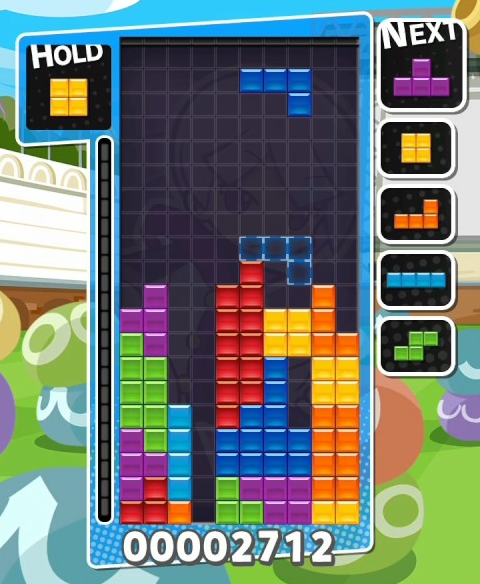
\includegraphics[scale=0.4]{imgs/tetris.png}
    \caption{Tetris}
    \label{fig:tetris}
\end{figure}

\begin{figure}[ht]
    \centering
    \begin{minipage}{.45\textwidth}
        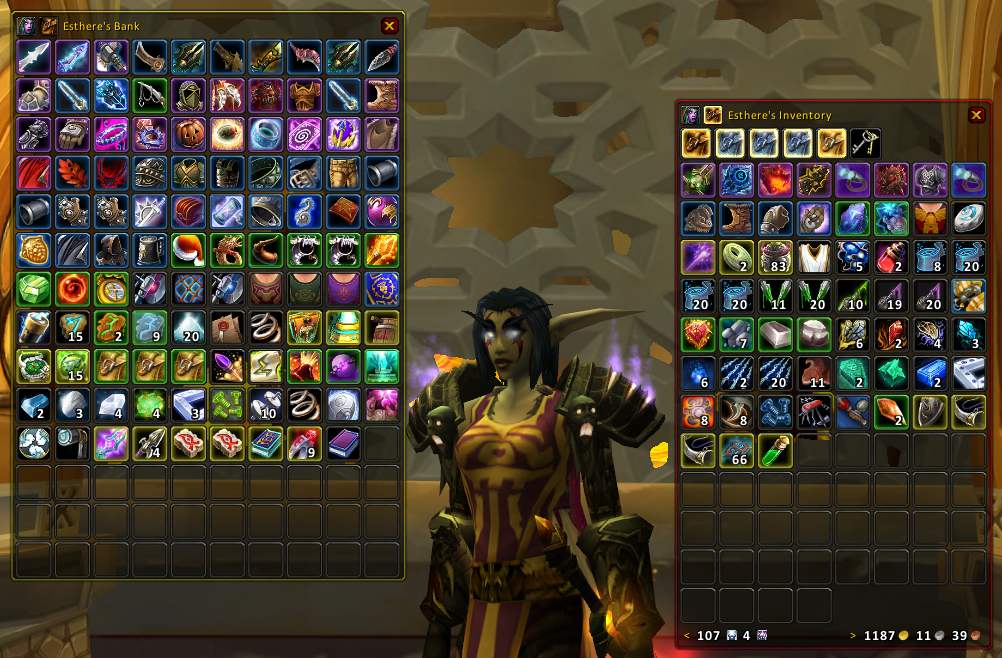
\includegraphics[width=\textwidth]{imgs/wow-inventory.png}
    \end{minipage}
    \begin{minipage}{.45\textwidth}
        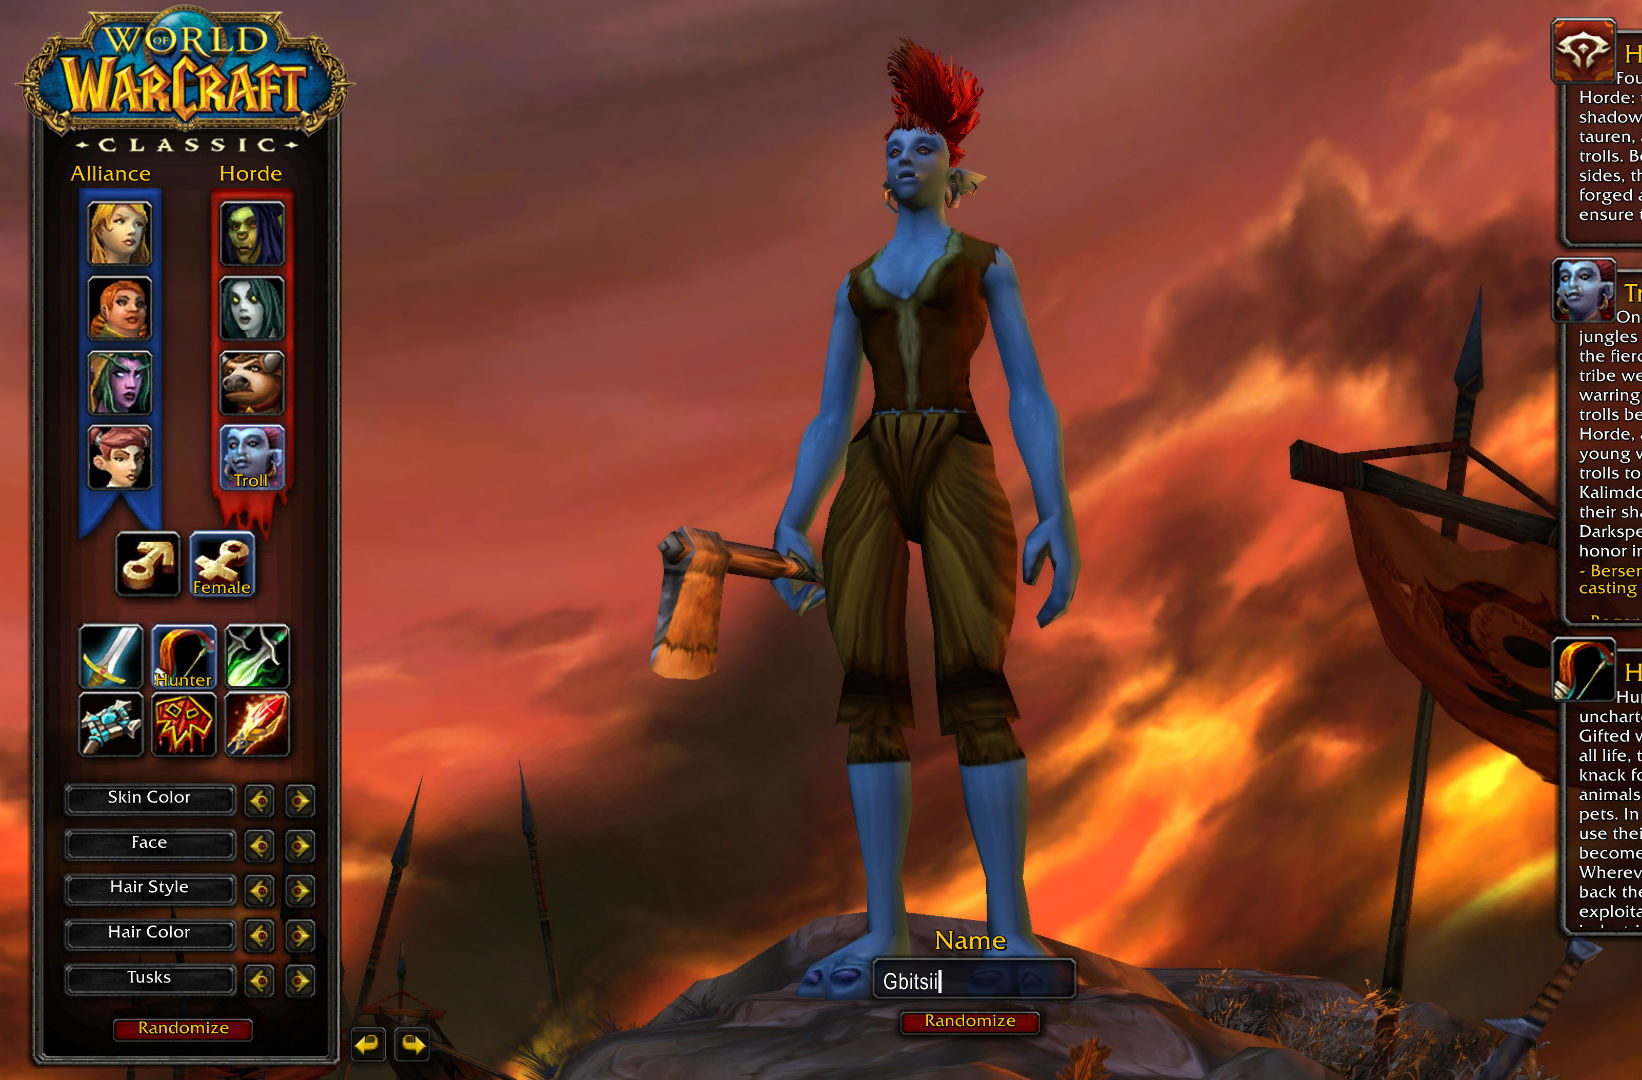
\includegraphics[width=\textwidth]{imgs/wow-class-choice.jpg}
    \end{minipage}
    \caption{World of Warcraft: Inventario y Elección de Clases}
    \label{multifig:wow}
\end{figure}

\begin{figure}[ht]
    \centering
    \begin{minipage}{.45\textwidth}
        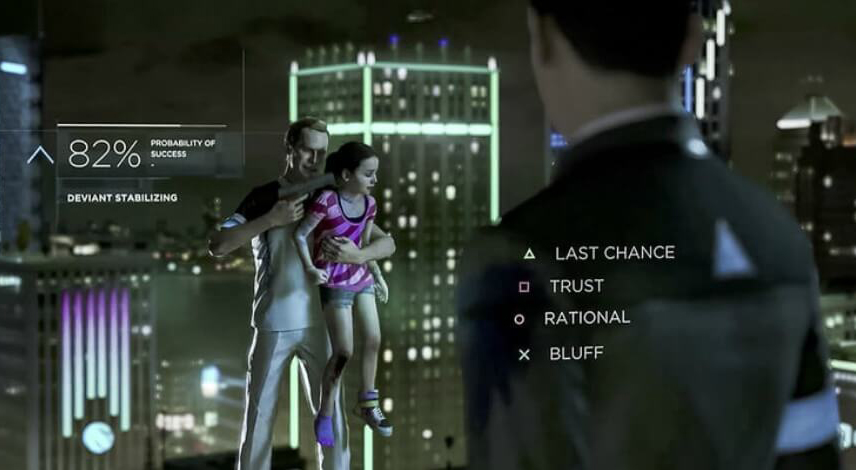
\includegraphics[width=\textwidth]{imgs/detroit-choices.jpg}
    \end{minipage}
    \begin{minipage}{.45\textwidth}
        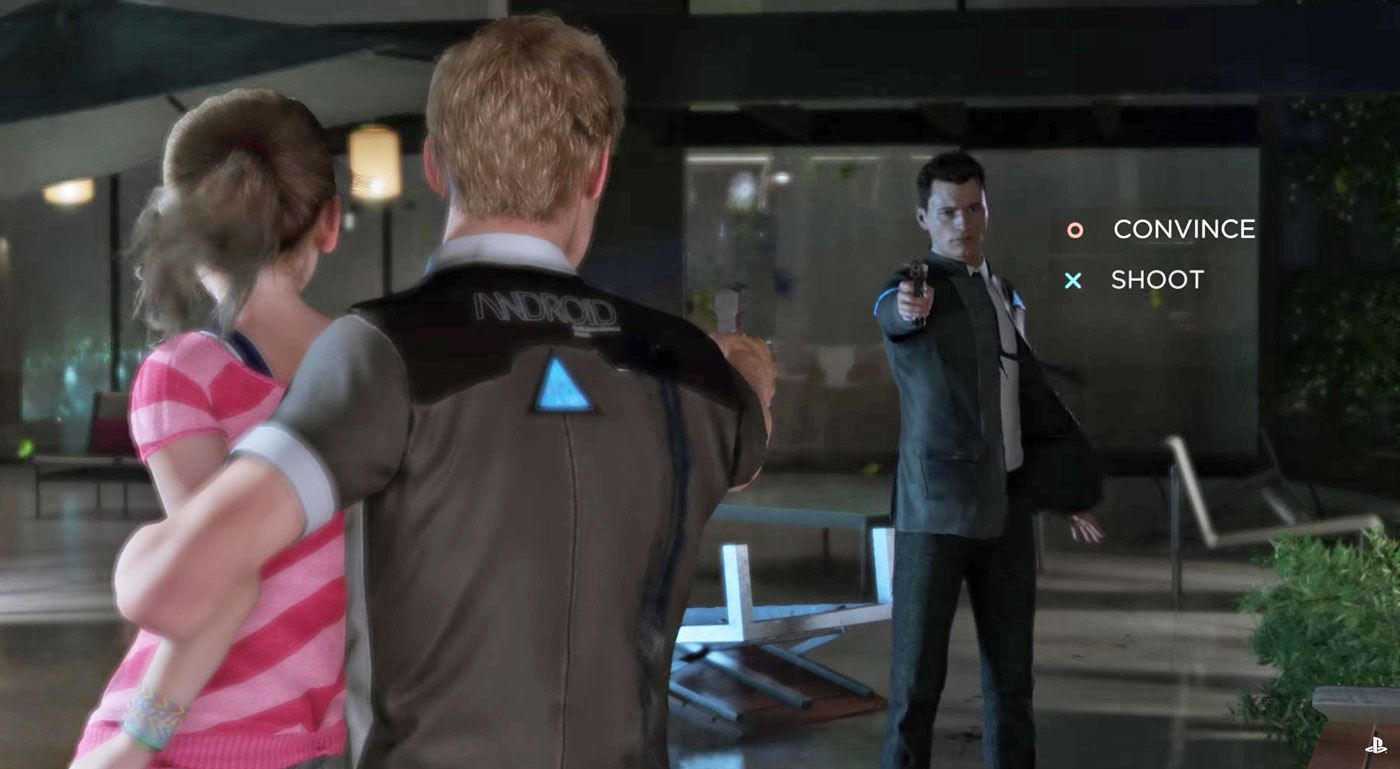
\includegraphics[width=\textwidth]{imgs/detroit-shoot.jpg}
    \end{minipage}
    
    \caption{Detroit Become Human}
    \label{multifig:detroit}
\end{figure}

La mayoría de este tipo de decisiones pueden ser superfluas para el jugador, o pueden importarle solamente para efectos de estrategia y para el contexto del juego. Sin embargo, determinados videojuegos pueden presentar dilemas morales que nos hacen reflexionar y ser más cautelosos con las decisiones que tomamos. No es lo mismo preguntarse si elegir una espada o un arco, a tener la vida de otra persona en tus manos, o que esa persona sea alguien con quien tenemos un vinculo cercano.

\subsection{Propósito}

El propósito de este proyecto es realizar una investigación respecto a los dilemas morales que los videojuegos pueden ofrecerle a los jugadores. Más precisamente, nos interesa saber si estos dilemas son significativos para el jugador a tal punto de llegar a cambiar su moral y su percepción sobre ciertos temas.


\subsection{Objetivo}

El objetivo de este proyecto es evaluar experimentalmente el impacto que los videojuegos y sus dilemas morales pueden tener sobre las personas.

Para alcanzar este objetivo se deberá:
\begin{itemize}
    \item Diseñar e implementar un videojuego en el que la toma de decisiones juegue un papel fundamental. Nos interesará que estas decisiones queden integradas en la historia del juego. Se le presentará un dilema moral inicial al jugador, y dependiendo de su respuesta, el videojuego y su historia trataran de influenciar al jugador para que cambie su opción.
    \item Diseñar y realizar un estudio con cuestionarios pre- y post- juego que nos permita analizar el comportamiento del jugador.
    \item Analizar los datos obtenidos en las sesiones de prueba para comprobar la hipótesis planteada y ver como el videojuego afectó a los jugadores.
\end{itemize}

\subsection{Distribución de tareas}

Dado que el videojuego creado para este proyecto es uno que trata de influenciar al jugador -para ver si podemos cambiar su decisión inicial- la componente narrativa es a la que más peso se le dará.

No obstante, el resto de las áreas no pueden quedar descuidadas ya que al formar parte de un todo, colaboran en la inmersión que tenga el jugador dentro de nuestro mundo y nuestra narrativa. Es de esperar que a mayor inmersión, mayor empatía por parte del jugador con la historia y más beneficioso será para los fines de nuestro proyecto.

Teniendo en cuenta estas consideraciones, el peso de las tareas para el desarrollo del videojuego queda determinado de la siguiente manera:

\begin{table}[H]
	\begin{center}
		\begin{tabular}{|>{\columncolor{Gray}}p{3cm}|p{3cm}|}
		\hline
		Estética 	& 20\% \\
		\hline
		Narrativa 	& 40\% \\
		\hline
		Mecánicas 	& 20\% \\
		\hline
		Tecnología 	& 20\% \\
		\hline
		\end{tabular}
		\caption{Distribución de las tareas - Videojuego}
		\label{tab:distribucion-videojuego}
	\end{center}
\end{table}

Además de esto, es necesario tener en cuenta también las tareas asociadas al estudio de los cuestionarios que se aplicarán pre- y post- juego, así como también la preparación del documento.

Considerando la investigación necesaria para ambos casos, podemos armar una tabla de pesos para el desarrollo del proyecto completo que quedaría de la siguiente manera:

\begin{table}[H]
    \centering
    \begin{tabular}{|>{\columncolor{Gray}}p{3cm}|p{3cm}|}
        \hline
        Videojuego &  50\%\\
        \hline
        Investigación & 20\%\\
        \hline
        Cuestionarios & 15\%\\
        \hline
        Documentación & 15\%\\
        \hline
    \end{tabular}
    \caption{Distribución de las tareas - General}
    \label{tab:destribucion-general}
\end{table}

